%%%%%%%%%%%%%%%%%%%%%%%%%%%%%%%%%%%%%%%%%%%%%%%%%%%%%%%%%%%%%%%%%%%%%%%%%
% This file is part of the LaTeX sources of the OMDoc 1.6 project descriptions
% Copyright (c) 2006 Serge Autexier, Dieter Hutter, Till Mossakowski, Axel Schairer
% This work is licensed by the Creative Commons Share-Alike license
% see http://creativecommons.org/licenses/by-sa/2.5/ for details
% The source original is at https://github.com/KWARC/OMDoc/doc/projects/maya
%%%%%%%%%%%%%%%%%%%%%%%%%%%%%%%%%%%%%%%%%%%%%%%%%%%%%%%%%%%%%%%%%%%%%%%%%

\begin{omgroup}[id=maya,short=Maya,creators={autexier,hutter,mossakowski,shairer}]
  {\maya: Maintaining Structured Developments}
\ednote{project page: \url{www.dfki.de/~inka/maya.html}}

\newcommand{\MAYAfigure}{%
  \begin{figure}[t]
    \begin{minipage}[t]{.79\textwidth}
      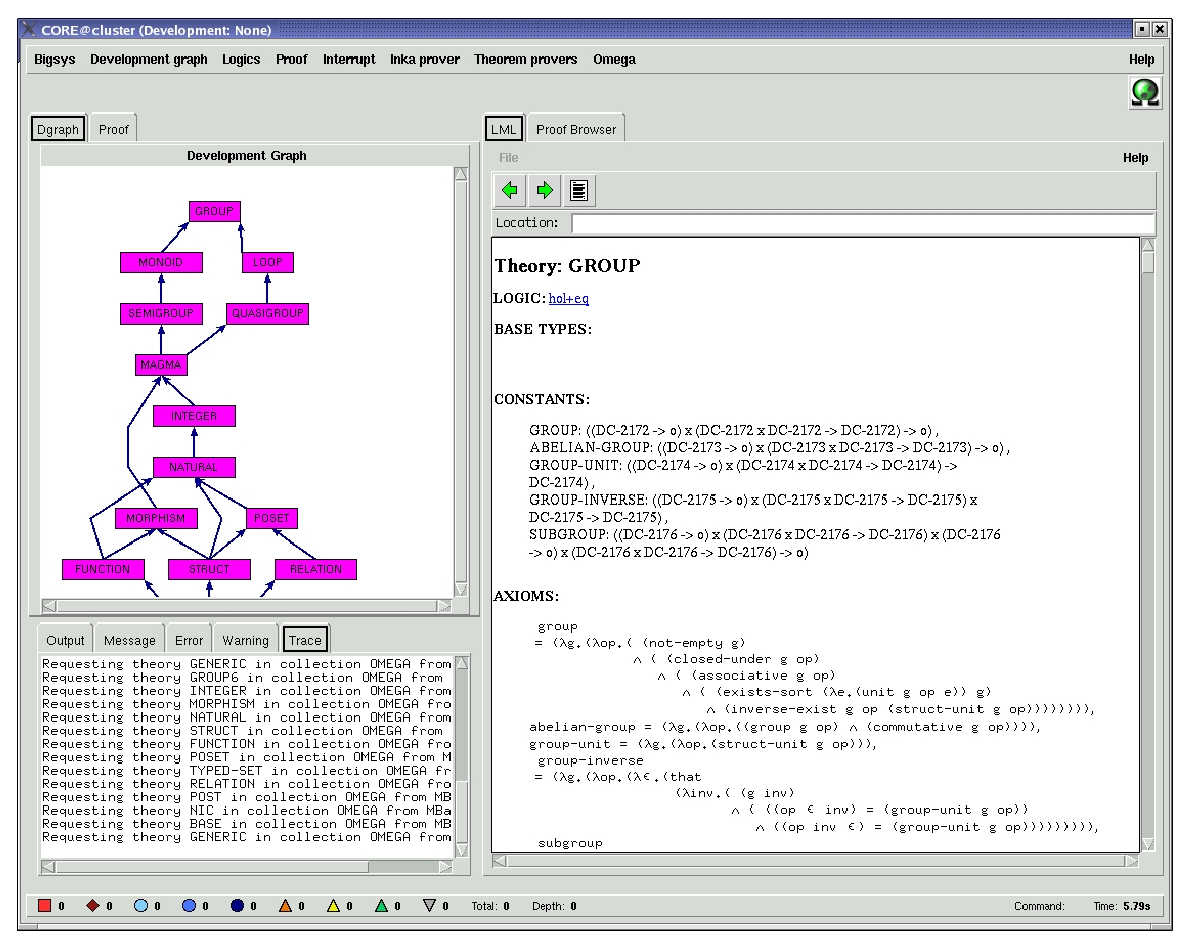
\includegraphics[width=.8\textwidth]{\projectsPath{maya/maya-screenshot}}
    \end{minipage}
    \hfill
    \begin{minipage}[b]{.15\textwidth}
      \hspace*{-1.7cm}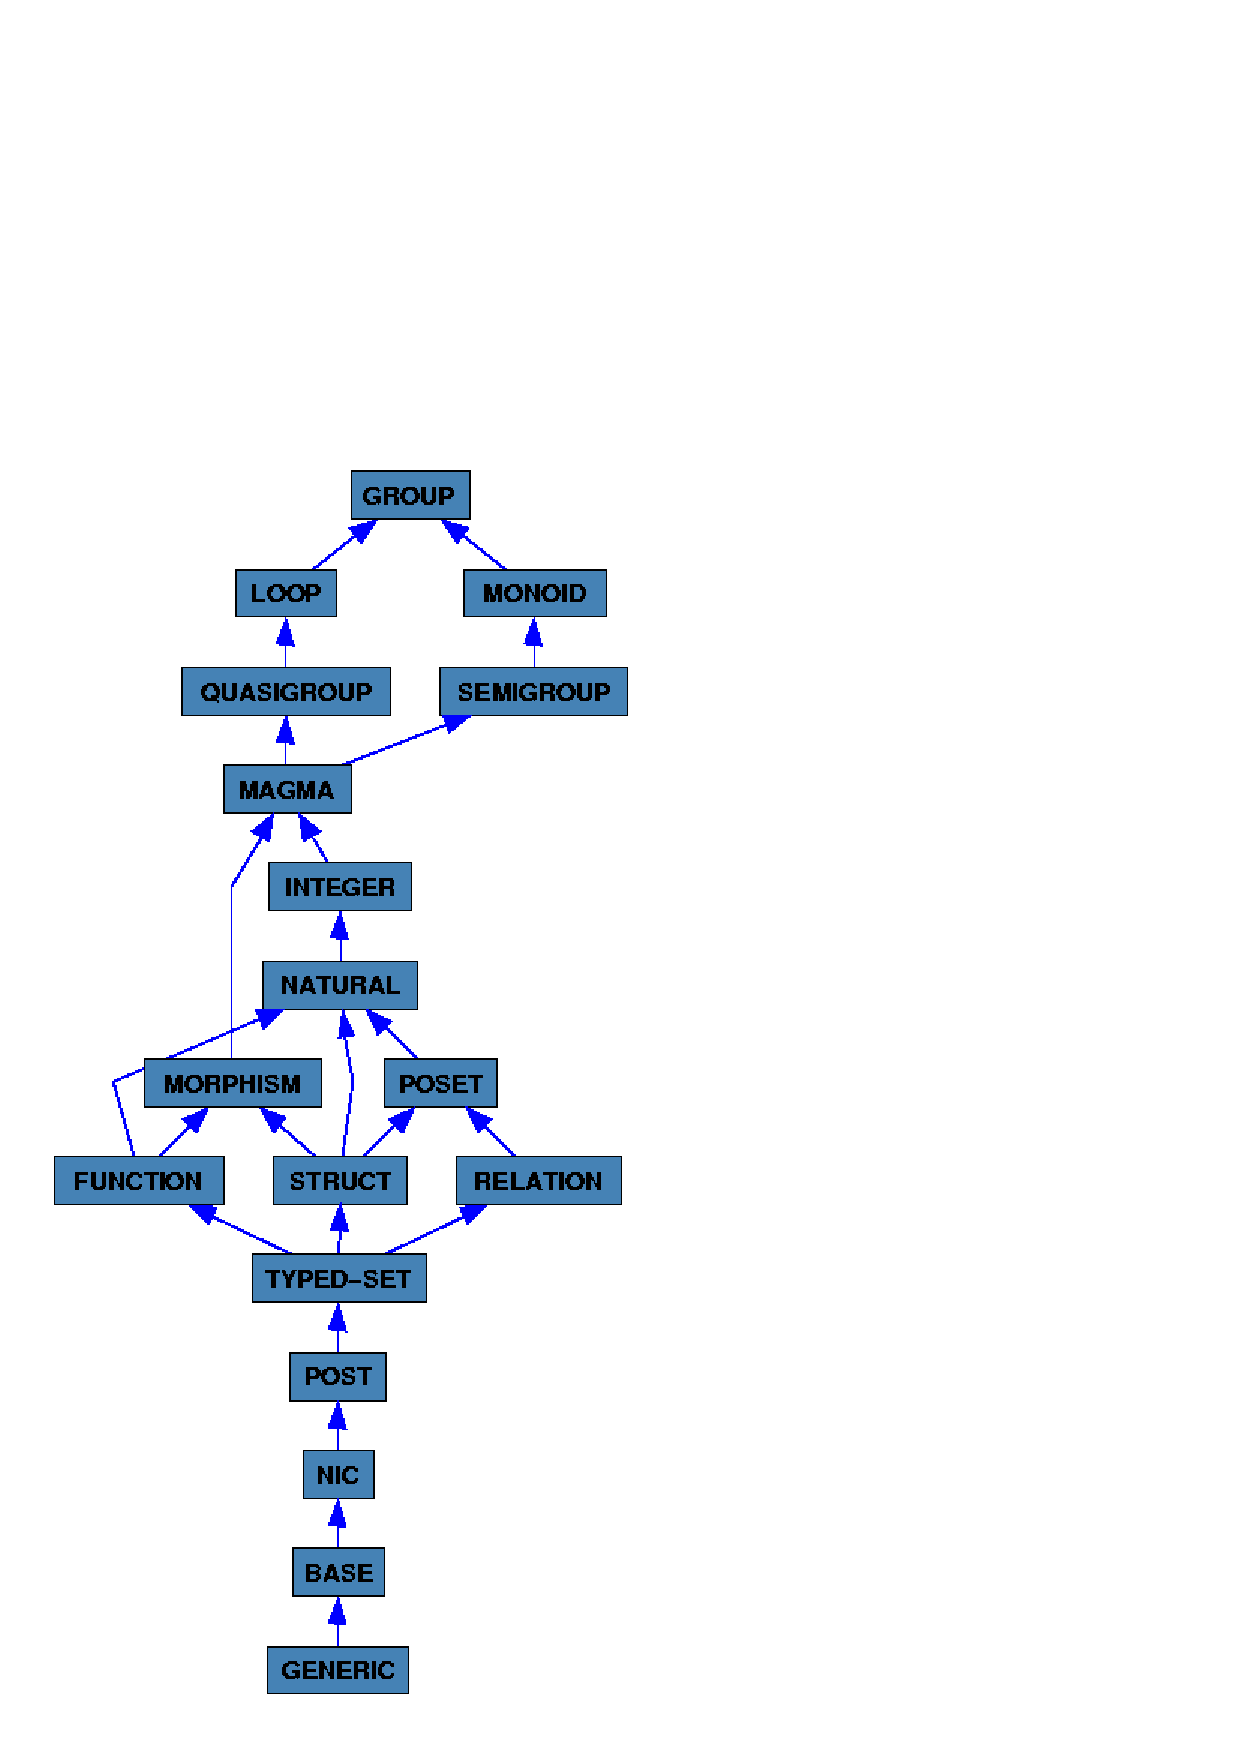
\includegraphics[width=1.25\textwidth]{\projectsPath{maya/omdoc-group}}
  \end{minipage}
  \caption{The graphical user interface of {\maya} \& the development graph for the {\omdoc} Representation of Groups in {\mbase}}\label{fig:maya-omdoc-group}
\end{figure}
}


\begin{omgroup}{Overview}

The {\maya}-system was originally designed to maintain and utilize the structuring
mechanisms incorporated in various specification
languages\twin{structured}{specifications} when evolving and verifying
{\atwintoo{formal}{software}{development}s}. In this setting, a software system as well as
their requirement specifications are formalised in a textual manner in some specification
language like {\casl}~\cite{CoFI:2004:CASL-RM} or {\vsesl}~\cite{VSE00}. All these
specification languages provide constructs similar to those of {\omdoc} to structure the
textual specifications and thus ease the reuse of
components\twin{component}{reuse}. Exploiting this structure, e.g.  by identifying
{\twintoo{shared}{component}s} in the {\twintoo{system}{specification}} and the
{\twintoo{requirement}{specification}}, can result in a drastic reduction of the
{\twintoo{proof}{obligation}s}, and hence of the {\twintoo{development}{time}} which again
reduces the overall project costs.

However, the logical formalisation of software systems is error-prone.  Since even the
verification of small-sized industrial developments requires several person months,
specification errors revealed in late verification phases pose an incalculable risk for
the overall project costs. An {\emph{evolutionary formal
    development}}\atwin{formal}{software}{development} approach is absolutely
indispensable. In all applications so far development steps turned out to be flawed and
errors had to be corrected. The search for formally correct software and the corresponding
proofs is more like a {\emph{formal reflection}} of partial developments rather than just
a way to assure and prove more or less evident facts.

The {\maya}-system supports an evolutionary formal development since it allows users to
specify and verify developments in a structured manner, incorporates a uniform mechanism
for verification {\emph{in-the-large}}\twin{verification}{in-the-large} to exploit the
structure of the specification, and maintains the verification work already done when
changing the specification. {\maya} relies on
{\emph{\twintoo{development}{graph}s}}~\cite{AH-05-a,Hutter:mocsv00} as a uniform (and
institution independent\footnote{This includes, for instance, that it does not require a
  particular logic (see e.g.~\cite{MAH-06-a} for more details).})  representation of
structured specifications, and which provide the logical basis for the {\emph{Complex
    theories}} and {\emph{Development graphs}} of {\omdoc}\footnote{These are the modules
  {\CTHmodule{spec}} and {\DGmodule{sped}}, respectively.}.  Relying on development graphs
enables {\maya} to support the use of various (structured) specification languages like
{\omdoc}, {\casl}~\cite{CoFI:2004:CASL-RM}, and {\vsesl}~\cite{VSE00} to formalise
mathematical theories\twin{mathematical}{theory} or
{\atwintoo{formal}{software}{development}s}.  To this end {\maya} provides a generic
interface to plug in additional parsers for the support of other specification languages.
Moreover, {\maya} allows the integration of different theorem provers to deal with the
actual {\twintoo{proof}{obligation}s} arising from the specification, i.e.  to perform
verification {\emph{in-the-small}}\twin{verification}{in-the-small}.

Textual specifications are translated into a structured logical representation called a
development graph, which is based on the notions of consequence relations and morphisms
and makes arising proof obligations explicit.  The user can tackle these proof obligations
with the help of theorem provers connected to {\maya} like Isabelle~\cite{Paulson:iagtp94}
or {\inka}~\cite{INKA5}.

A failure to prove one of these obligations usually gives rise to modifications of the
underlying specification.  {\maya} supports this {\twintoo{evolutionary}{process}} as it
calculates minimal changes to the logical representation readjusting it to a modified
specification while preserving as much verification work as possible.  If necessary it
also adjusts the database of the interconnected theorem prover.  Furthermore, {\maya}
communicates explicit information how the axiomatization has changed and also makes
available proofs of the same problem (invalidated by the changes) to allow for a reuse of
proofs inside the theorem provers. In turn, information about a proof provided by the
theorem provers is used to optimise the maintenance of the proof during the evolutionary
development process.
\end{omgroup}

\begin{omgroup}{From Textual to Logical Representation}

The specification of a formal development in {\maya} is always done in a textual way using
specification languages like {\casl} , {\omdoc} or {\vsesl}.  {\maya} incorporates parsers
to translate such specifications into the {\maya}-internal specification language {\dgrl}
(``Development Graph Representation Language'').  {\dgrl} provides a simply-typed
$\lambda$-calculus to specify the local axiomatization of a theory in a
{\twintoo{higher-order}{logic}}. While unstructured specifications are solely represented
as a signature together with a set of logical formulas, the structuring operations of the
specification languages are translated into the structure of a
{\twintoo{development}{graph}}. Each node of this graph corresponds to a
{\indextoo{theory}}. The axiomatization of this theory is split into a local part which is
attached to the node as a set of higher-order formulas and into global parts, denoted by
ingoing definition links, which import the axiomatization of other nodes via some
{\twintoo{consequence}{morphism}s} (such as the {\element{imports}} element in {\omdoc}).
While a {\emph{local}}\twin{local}{link} link imports only the local part of the
axiomatization of the source node of a link, {\emph{global}}\twin{link}{global} links are
used to import the entire axiomatization of
%%
\MAYAfigure
%%
a source node (including all the imported axiomatization of other nodes).  In the same
way local and global {\emph{theorem link}s} are used to postulate relations between nodes
(see~\cite{AH-05-a} for details) which correspond to {\omdoc}'s
{\element{theory-inclusion}} and {\element{axiom-inclusion}} elements.

On the left hand side, {\myfigref{maya-omdoc-group}} shows the graphical user interface of
{\maya}. The right hand side shows the development graph in {\maya} for a formalisation of
groups. The formalisation was given in {\omdoc} and imported into {\maya} from the
{\omdoc} database {\mbase} (see~\cite{KohFra:rkcimss01} and {\sref{mbase}}).
\end{omgroup}

\begin{omgroup}{Verification In-the-large}

The development graph is the central data-structure to store and maintain the formal
(structured) specification, the arising {\twintoo{proof}{obligation}s} and the status of
the corresponding verification effort (proofs) during a formal development.

{\maya} distinguishes between proof obligations postulating properties between different
theories (like the {\element{theory-inclusion}} and {\element{axiom-inclusion}} elements
in {\omdoc}) and lemmata postulated within a single theory (like {\element{assertion}} in
{\omdoc}).  As theories correspond to subgraphs within the development graph, a relation
between different theories, represented by a {\atwintoo{global}{theorem}{link}},
corresponds to a relation between two subgraphs.  Each change of these subgraphs can
affect this relation and would invalidate previous proofs of this relation. Therefore,
{\maya} decomposes relations between different theories into individual relations between
the local axiomatization of a node and a theory (denoted by a local theorem link). Each of
these relations decomposes again into a set of {\twintoo{proof}{obligation}s} postulating
that each local axiom of the node is a theorem in the target theory with respect to the
morphism attached to the link.

While definition links establish relations between theories, theorem links denote
lemmata postulated about such relations. Thus, the reachability between two nodes
establishes a formal relation between the connected nodes (i.e. the theory of the
source node is part of the theory of the target node wrt. the morphisms attached
to the connecting links). {\maya} uses this property to prove relations between
theories by searching for paths between the corresponding nodes (instead of
decomposing the corresponding proof obligation in the first place).
\end{omgroup}

\begin{omgroup}{Verification In-the-small}

When verifying a local theorem link or proving speculated lemmata, the conjectures have to
be tackled by some interconnected theorem prover.  In both cases the proofs are done
{\emph{within}} a specific theory.  Thus, conceptually each theory may include its own
theorem prover.  In principle, there is a large variety of
{\twintoo{integration}{type}s}. The tightest integration consists of having a theorem
prover for each node wrt.  which theory conjectures must be proven, and the theorem prover
returns a proof object generated during the proof of a conjecture.  Those are stored
together with the conjecture and can be used by {\maya} to establish the validity of the
conjecture if the specification is changed. The loosest integration consists in having a
single generic theorem prover, which is requested to prove a conjecture within some theory
and is provided with the axiomatization of this theory. The theorem prover only returns
whether it could prove a conjecture or not, without any information about axioms used
during the proof. For a detailed discussion of the advantages and drawbacks of the
different integration scenarios see~\cite{AutMos:ihdgmm02}.

Currently, {\maya} supports two integration types: One where
information about used axioms is provided by the theorem prover, and
one where no such information is provided. In the first case, {\maya}
stores the proof information and the axioms used during the proof. In the second
case, {\maya} assumes there is a proof for the proof obligation, as there is no
information about the proof. In both scenarios, {\maya} makes use of
generic theorem provers which are provided with the axiomatization of
the current theory. Currently {\maya} provides all axioms
and lemmata located at theories that are imported from the actual theory
by definition links to the prover. Switching between different proof obligations may
cause a change of the current underlying theory and thus a change of
the underlying axiomatization.  {\maya} provides a generic interface to
plug in theorem provers (based on an XML-RPC protocol) that allows for
an incremental update of the database of the prover.
\end{omgroup}

\begin{omgroup}{Evolution of Developments}

The user executes changes to specifications in their textual representation.  Parsing a
modified specification results in a modified {\dgrl}-specification. In order to support a
{\twintoo{management of}{change}}, {\maya} computes the differences of both
{\dgrl}-specifications and compiles them into a sequence of basic operations in order to
transform the {\twintoo{development}{graph}} corresponding to the original
{\dgrl}-specification to a new one corresponding to the modified
{\dgrl}-specification. Examples of such basic operations are the insertion or deletion of
a node or a link, the change of the annotated morphism of a link, or the change of the
local axiomatization of a node. As there is currently no optimal solution to the problem
of computing differences between two specifications, {\maya} uses heuristics based on
names and types of individual objects to guide the process of mapping corresponding parts
of old and new specification. Since the differences of two specifications are computed on
the basis of the internal {\dgrl}-representation, new specification languages can easily
be incorporated into {\maya} by providing a parser for this language and a translator into
{\dgrl}.

The development graph is always synthesised or manipulated with the help of the
previously mentioned basic operations (insertion\slash deletion\slash change of
nodes\slash links\slash axiomatization) and {\maya} incorporates sophisticated
techniques to analyse how these operations will affect proof obligations or proofs
stored within the development graph. They incorporate a notion of monotonicity of
theories and morphisms, and take into account the sequence in which objects are
inserted into the development graph. Furthermore, the information about the
decomposition and subsumption of global theorem links obtained during the
verification {\emph{in-the-large}}\twin{verification}{in-the-large} is explicitly
maintained and exploited to adjust them once the development graph is altered.
Finally, the knowledge about proofs, e.g. the used axioms, provided by the
interconnected theorem provers during the verification
{\emph{in-the-small}}\twin{verification}{in-the-small} is used to preserve or
invalidate the proofs.
\end{omgroup}

\begin{omgroup}{Conclusion and System Availability}

The {\maya}-system is mostly implemented in Common Lisp while parts of the GUI, shared
with the {\OMEGA}-system~\cite{SieHes:loui99}, are written in Mozart. The {\casl}-parser
is provided by the CoFI-group in Bremen (see {\sref{hets}}). The {\maya}-system is
available from the {\maya}-web-page at {\url{http://www.dfki.de/~inka/maya.html}}.

The Heterogeneous Tool Set ({\hets}, see \sref{hets}) extends {\maya} with a treatment
of hiding~\cite{MAH-06-a}, and a uniform treatment of different logics based on the notion
of heterogeneous development graphs~\cite{Mossakowski:tdghb02}.  Furthermore, it is planned
to extend this with the maintenance of theory-specific control information for theorem
provers. The latter comprises a management for building up the database of theorem provers
by demand rather than providing all available axioms and lemmata at once and it comprise
the management of meta-level information, like tactics or proof plans, inside {\maya}.
\end{omgroup}
\end{omgroup}
% LocalWords:  Stuhlsatzenhausweg FASE Hutter Mossakowski Inka maya Saarbr wrt
% LocalWords:  Schairer Informatik Isabelle Dgrl lemmata CoFI inka Autexier
% LocalWords:  DKFI GmbH autexier hutter schairer dfki ucken omdoc mbase hets
%%% Local Variables: 
%%% mode: latex
%%% TeX-master: "../main"
%%% End: 
